% Chapter 1

\chapter{Evaluation} % Main chapter title

\label{Chapter4} % For referencing the chapter elsewhere, use \ref{Chapter1} 

\lhead{Chapter 4. \emph{Evaluation}} % This is for the header on each page - perhaps a shortened title

%----------------------------------------------------------------------------------------
\noindent In this chapter we validate and evaluate our designs. Validation is important to prove that our approach works and evaluation -- to analyze how good it performs.

\section{Approach Validation}

\noindent First, to validate the whole application provisioning and deployment approach, we have to refer back to the requirements defined in Section 2. The two requirements that were not satisfied by the CloudMF approach were: (i) a domain-specific workflow definition language to describe deployment plans and (ii) possibility to refine the default deployment plan. With the creation of the deployment and provisioning DSL and an internal DSL to manipulate the deployment plans, we can safely state that both requirements are satisfied now. 

\noindent Next, to actually validate our approach, several applications were deployed:

\begin{enumerate}
\item  Storm cluster, which was described in the motivating example and consists of nimbus node, zookeeper node and supervisor node.

\item  SensApp \footnote{ SensApp 1 VM, https://github.com/SINTEF-9012/cloudml/blob/master/docs/samples/sensapp-v2.json}(1 VM): is an open-source application for storing and exploiting data sets collected from different sensors. In this application topology model all SensApp components are installed on one virtual machine.

\item  SensApp\footnote{ SensApp 2 VMs, https://github.com/SINTEF-9012/cloudml/blob/master/docs/samples/sensappAdmin-v2.json} (2 VMs): SensApp admin component is hosted on another virtual machine. The deployment plan for a SensApp with two virtual machines was depicted on Figure 15. 
\end{enumerate}

\noindent All deployments were performed on a Windows 7, 64-bit OS with Intel Core i7-3520M processor and 8 GB of RAM, with such resource consuming applications as Google Chrome web browser and Intellij Idea IDE running at the same time. 

\noindent The Storm cluster application was chosen for experiments because it is a good example of a distributed application with a master-slave architecture. While each component of a Storm cluster is hosted on a separate VM, every VM has only one component installed. That is why SensApp application was taken for the second experiment -- in SensApp the software stack is more complex and there are more dependencies between different components. Finally, SensApp with two VMs was chosen to show how bursting out scenarios could be achieved with our approach. For instance, SensApp admin component could have a policy that it needs a certain amount of CPU to be available for proper operation. When the policy threshold would be reached, a reasoning engine could update the application topology model and redeploy SensApp application. After the redeployment, SensApp application would be running on one VM, and SensApp admin -- on another. Because CloudMF does not support policies yet, we simply updated the model by hand and executed redeployment.

%----------------------------------------------------------------------------------------
\section{Approach Evaluation}

\noindent In addition to the aforementioned deployments, we evaluated several deployment execution approaches in terms of the response time: sequential, parallel and concurrent execution of tasks. The results of our experiments are shown in Table \ref{tab:3}. On Figure \ref{fig:algorithms} we can clearly see that the concurrent algorithm is the fastest one in all three cases. In addition, considering the result depicted in the Figure \ref{fig:sensapp_times}, when the number of the application's components increases (SensApp with 2 VMs with respect to the SensApp with 1 VM), the execution time of the sequential approach obviously increases too, whilst when using the parallel approach it decreases. 

\begin{center}	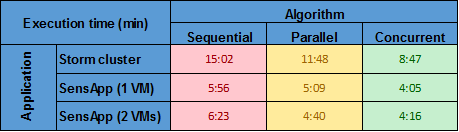
\includegraphics{./Figures/deployment_times}
	\begin{table}[htbp]
    \caption{Application Deployment Times}
    \label{tab:3}
	\end{table}
\end{center} 

\noindent 

\begin{figure}[htbp]
	\centering	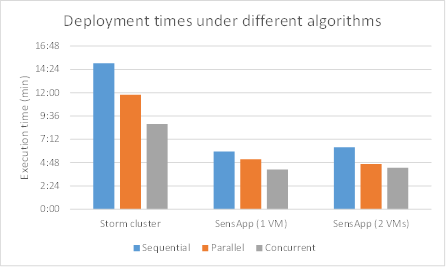
\includegraphics{./Figures/deployment_comparison}
		\rule{38em}{0.5pt}
	\caption[Comparison of Algorithms]{Comparison of deployment algorithms}
	\label{fig:algorithms}
\end{figure}

\noindent 

\begin{figure}[htbp]
	\centering	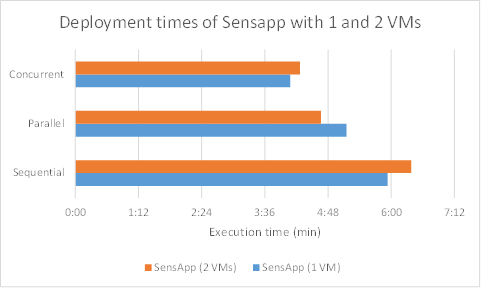
\includegraphics{./Figures/deployment_sensapp}
		\rule{38em}{0.5pt}
	\caption[Comparison of SensApp Execution Times]{Comparison of deployment algorithms when number of application components is growing}
	\label{fig:sensapp_times}
\end{figure}

\noindent 

\begin{figure}[htbp]
	\centering	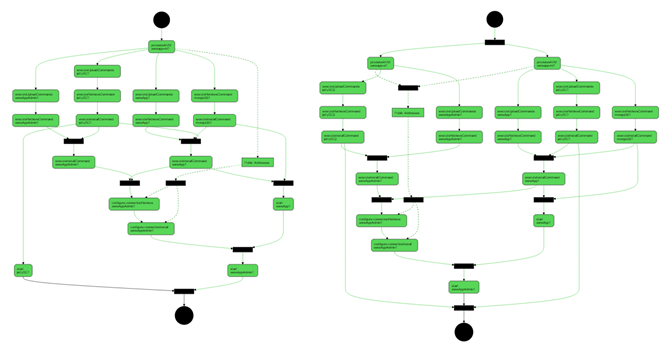
\includegraphics[width=38em]{./Figures/two_vms}
		\rule{38em}{0.5pt}
	\caption[SensApp Deployment Plans]{Deployment plans of the SensApp with 1 VM (left) and 2 VMs (right)}
	\label{fig:sensapp_plans}
\end{figure}

\noindent The reason for that is that bigger number of components, and in particular VMs, allowed the application to utilize parallel threads more efficiently, so the overall deployment time decreased. This can be observed from the Figure \ref{fig:sensapp_plans} where the number of tasks on the deployment plan at the right side of the figure is bigger, but at the same time it has more parallel branches.

\noindent One would expect the same behavior for the concurrent algorithm. Instead, the deployment time under concurrent execution slightly increased. A possible reason for that could be in the structure of the deployment plan. If the plan is relatively symmetric, it does not matter much if one branch can be executed faster than another because they have similar number of tasks (assuming those tasks have similar execution times). In such cases parallel algorithms could probably achieve maximum performance. In scenarios where the plan structure is unbalanced, the number of tasks in every branch differs significantly or there are many forks and joins, independent execution of tasks becomes more important, so concurrent algorithms shall be favored. These are just assumptions, to give a definite answer, a bigger number of experiments with different application topology structures shall be conducted. Moreover, it is out of scope of this work to evaluate efficiency of graph traversal algorithms.

\noindent Another part of evaluation is related to the continuous deployment of cloud applications. We will refer to previous examples: SensApp application with one and two virtual machines. We already know the execution time of the SensApp deployment with two VMs, so the next step is to perform an adaptation: transition from the SensApp application with one VM to SensApp with two VMs. Figure \ref{fig:sensapp_adaptation} shows generated deployment plans in the case of full redeployment (left) and using the CloudML diff engine (right). The execution times and speed-up factors (the ratio between full redeployment and the diff approach) are shown in Table \ref{tab:4}. It may seem strange that execution times for the diff approach are the same under different algorithms, but it can be easily explained if we take a look at the deployment plan in the right part of Figure \ref{fig:sensapp_adaptation}. Two of the most time consuming tasks (installation of the Jetty server and SensApp admin component) has to be executed one after another, while other tasks are performed almost instantaneously. Consequently, the speed-up factor is the biggest for the sequential scenario because there is almost no parallelism and the benefits of parallel and concurrent algorithms can not be exploited.

\begin{center}	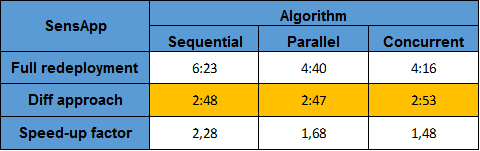
\includegraphics{./Figures/diff}
	\begin{table}[htbp]
    \caption{Evaluation of the Diff Approach}
    \label{tab:4}
	\end{table}
\end{center} 

\begin{figure}[htbp]
	\centering	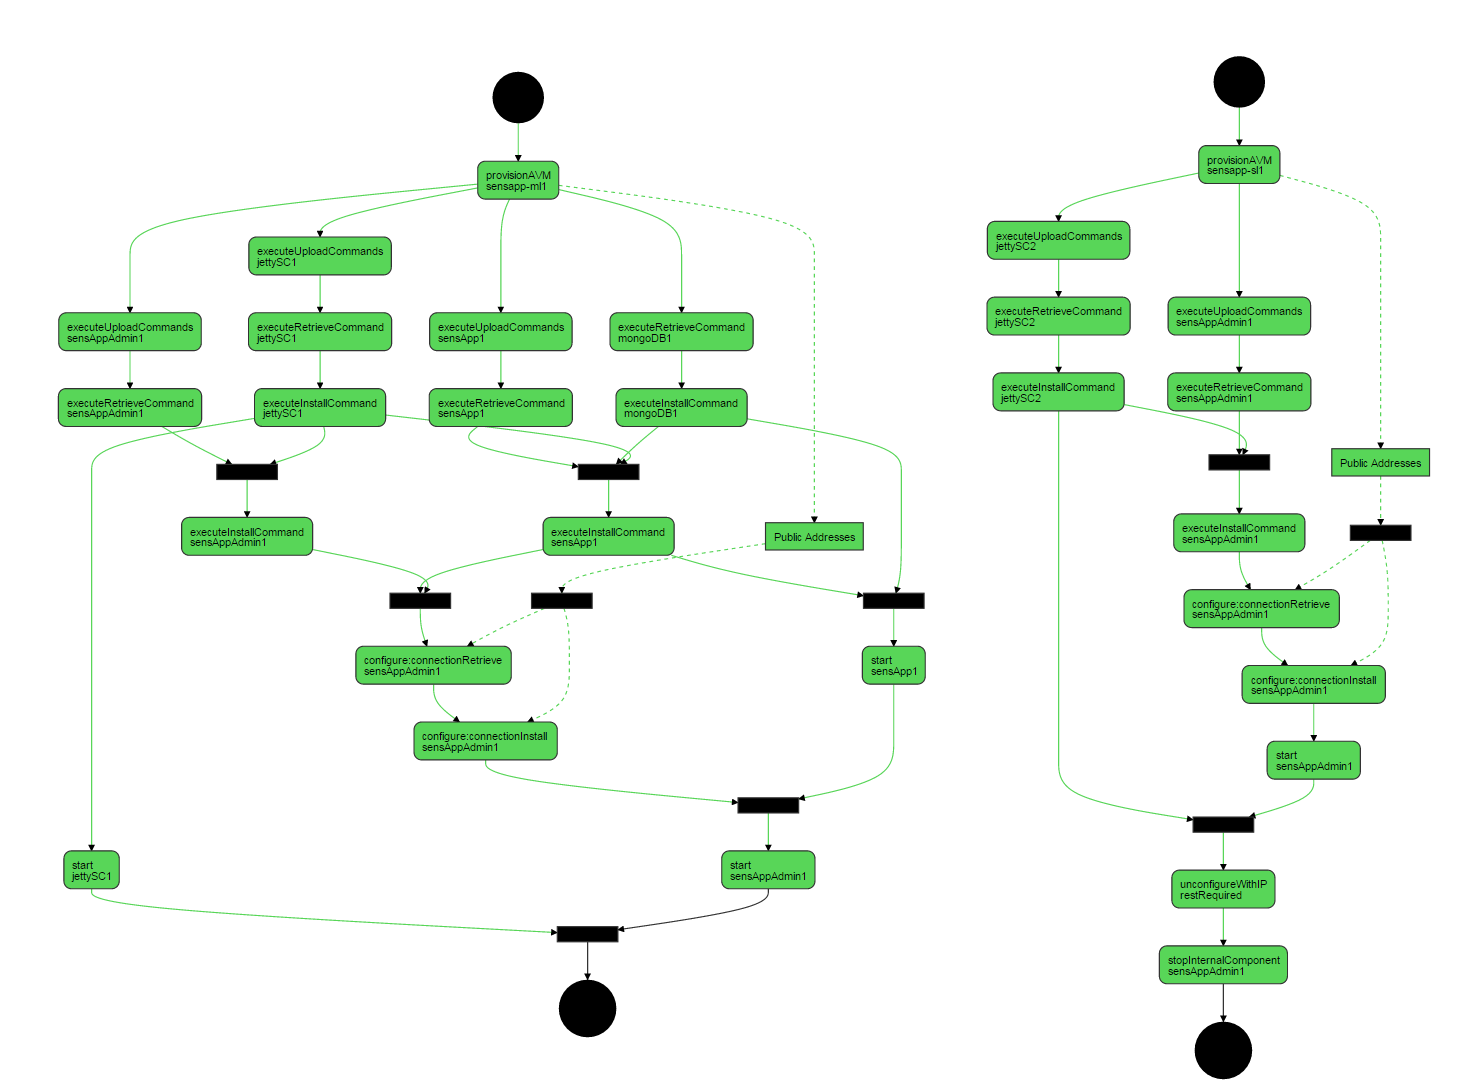
\includegraphics[width=38em]{./Figures/Sensapp_diff}
		\rule{38em}{0.5pt}
	\caption[SensApp Adaptation]{Sensapp (2VMs) deployment plans: full redeployment (left), diff approach (right)}
	\label{fig:sensapp_adaptation}
\end{figure}

\noindent

\noindent The real benefit of the diff approach comes in situations when adaptation plans are quite complex and affect a big part of the application topology. Benefits are achieved in terms of time as shown in the Table \ref{tab:4}, as well as in terms of complexity: the adaptation plan in Figure \ref{fig:sensapp_adaptation} is much simpler than the plan to redeploy the whole application. Simpler adaptation plans are also beneficial in the debugging scenarios -- they are easier to analyze and tune in case something goes wrong. Unfortunately, at the time of writing of this work we did not have application topology models of sufficient complexity to properly highlight the benefits of the diff approach. From the other side, it is intuitive that applying changes only to some part of the application would be faster than redeploying the whole application, especially in the large-scale setups. 

\noindent Finally, we would like to build up on the idea of the combination of parallel and concurrent graph traversal algorithms. If our assumptions, that parallel algorithms are more efficient on symmetric graphs and concurrent -- on asymmetric, are true, then a smart deployment engine could evaluate the deployment plan structure and then apply one or another graph traversal algorithm. A simple idea for evaluation if the graph is symmetric could be to mark graph nodes and edges with levels (as it is currently done in the parallel algorithm) and then compare number of tasks on all levels. If more than half levels have N parallel tasks (N $>$ 2), we could assume the plan is relatively symmetric and apply parallel execution algorithm, otherwise -- concurrent.
